%\clearpage
\section{Робот Rover Vehicle}
\subsection{Обзор робота}
Автомобиль TETRIX PRIME Rover -- это универсальная и увлекательная отправная
точка для различных проектов в области мехатроники и робототехники.
Это наземное транспортное средство, управляемое myRIO и оснащенное
двигателями и датчиками. Вы можете начать, следуя инструкциям по
сборке ровера и запустив предоставленный код. Это позволит вам
удаленно управлять марсоходом для перемещения и захвата объектов с помощью его
эффектора на конце клешни. Вы можете расширить функциональность ровера
, чтобы он мог использовать алгоритмы управления и выполнять задачи.

\subsection{Описание робота}
Два передних колеса приводятся в движение независимо друг от друга двигателями постоянного тока. Заднее колесо используется для балансировки и может свободно вращаться.
Скорость двигателей постоянного тока регулируется с помощью ШИМ, а их направление контролируется с помощью цифровой линии (эта проводка выполняется для вас через плату двигателя).
Ровер имеет дифференциальное рулевое управление, что означает, что направление движения ровера можно изменять, изменяя относительную скорость вращения двигателей постоянного тока.
Данные инфракрасного (ИК) дальномера считываются по аналоговой линии и преобразуются в сантиметры. Его можно использовать для определять расстояние до других объектов или различать различия в цвете и материале на основе ИК-отражательной способности.
Концевой эффектор клещей управляется серводвигателем. Положение серводвигателя контролируется с помощью ШИМ.
AM будет развернут в myRIO, что позволит ему выводить сигналы двигателя, вводить данные датчиков и передавать данные на главный компьютер и с него через сеть WI-Fi.

\newpage
\subsection{Сборка робота}
\begin{figure}[h]
    \begin{subfigure}[b]{0.45\textwidth}
        \centering
        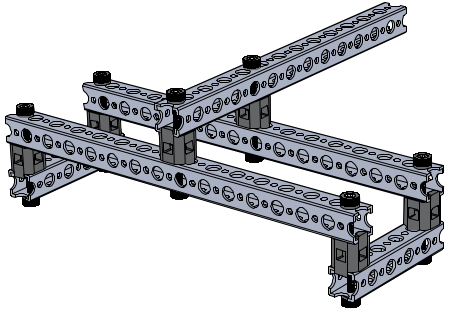
\includegraphics[width=0.7\textwidth]{fig/assembly/1.1.png}
        \caption*{Шаг 1}
    \end{subfigure}
    \begin{subfigure}[b]{0.45\textwidth}
        \centering
        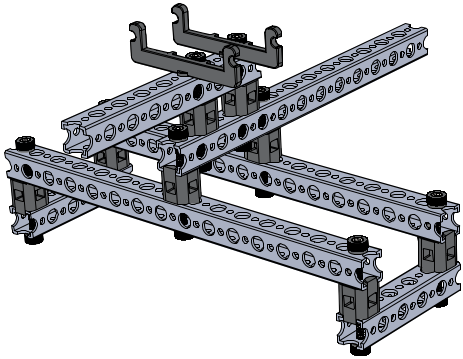
\includegraphics[width=0.7\textwidth]{fig/assembly/1.2.png}
        \caption*{Шаг 2}
    \end{subfigure}
    \begin{subfigure}[b]{0.45\textwidth}
        \centering
        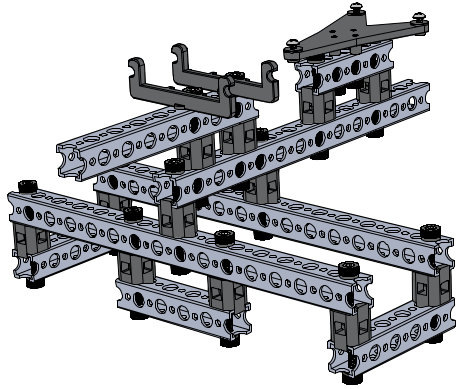
\includegraphics[width=0.7\textwidth]{fig/assembly/1.3.png}
        \caption*{Шаг 3}
    \end{subfigure}
    \begin{subfigure}[b]{0.45\textwidth}
        \centering
        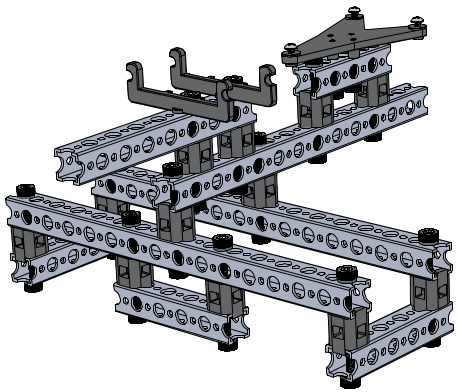
\includegraphics[width=0.7\textwidth]{fig/assembly/1.4.png}
        \caption*{Шаг 4}
    \end{subfigure}
    \begin{subfigure}[b]{0.45\textwidth}
        \centering
        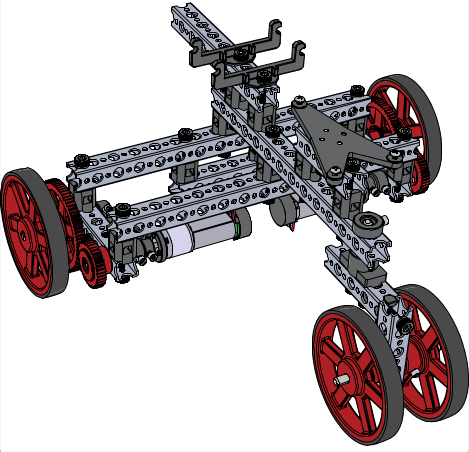
\includegraphics[width=0.7\textwidth]{fig/assembly/1.5.png}
        \caption*{Шаг 5}
    \end{subfigure}
    \begin{subfigure}[b]{0.45\textwidth}
        \flushright
        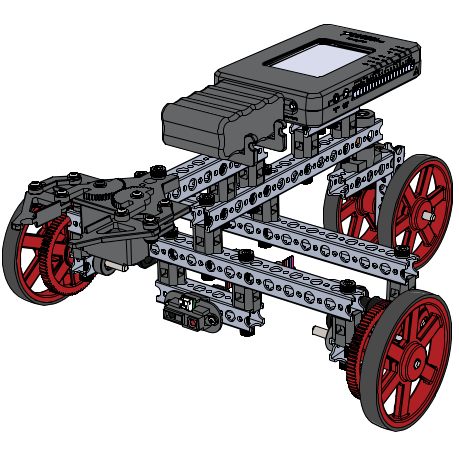
\includegraphics[width=0.7\textwidth]{fig/assembly/1.6.png}
        \caption*{Шаг 6}
    \end{subfigure}
\end{figure}

\newpage
\subsection{Подключение робота}
Подключение робота представлено на рисунке \ref{1connect}.
\begin{figure}[h]
    \centering
    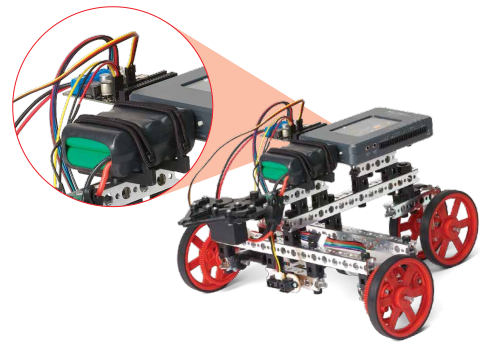
\includegraphics[width=0.7\textwidth]{fig/assembly/1.7.png}
    \caption{Подключение двигателей и периферии}
    \label{1connect}
\end{figure}

\subsection{Испытание робота}
Система управления с замкнутой обратной связью использует контур отрицательной обратной связи с датчиком для измерения выходного сигнала и
сравнения измеренного выходного сигнала, представленного Y (s), с эталонным входом, представленным R (s), для генерации сигнала
ошибки, представленного Ea (s), который управляет контроллер. Если мы сможем надлежащим образом использовать сигнал ошибки, то
достигнем нашей цели отслеживания, то есть сведем к минимуму E(s) =Y(s)-R(s) при наличии внешних помех и установки
неопределенности и изменения параметров. Это ключевая цель разработки контроллера с обратной связью с замкнутым контуром. ИК-датчик
может использоваться для различения цветов на основе различий в отражательной способности ИК-излучения для отслеживания предписанного пути, отмеченного на
земле. Он также может измерять расстояние до препятствий, позволяя нам пропускать препятствия или отслеживать предписанный путь через
загражденную область. С введением датчика мы получаем дополнительный нежелательный шум датчика, представленный
N (s). Основные преимущества управления с замкнутым контуром включают (i) повышенную надежность работы с замкнутым контуром до
изменения параметров установки, (ii) улучшенное подавление внешних помех, ослабление шума измерений
и уменьшение установившейся ошибки системы, и (iii) готовый контроль и регулировка переходной характеристики
системы благодаря умелой конструкции контроллера. Однако эти преимущества сопряжены с затратами. Основная стоимость
управления с обратной связью по замкнутому контуру заключается в дополнительной сложности, что означает более высокие денежные затраты и большую вероятность
отказов компонентов. Поскольку преимущества намного перевешивают недостатки, мы обнаруживаем, что управление с обратной связью по замкнутому контуру широко используется
в современных системах управления. Ключом к управлению с обратной связью по замкнутому контуру является использование сигнала ошибки отслеживания для улучшения
переходной характеристики (время установления, процент превышения и т.д.), а также уменьшения ошибок отслеживания ошибок в установившемся режиме.
Управляющая программа робота представлена на рисунке \ref{1prog}.
\begin{figure}[h]
    \centering
    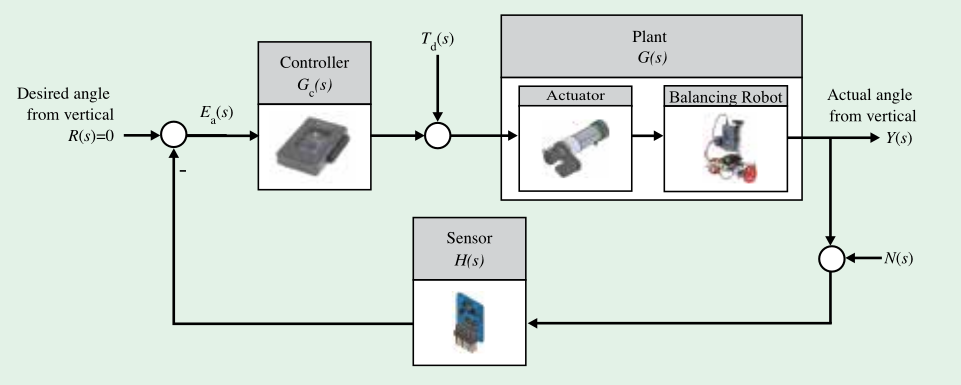
\includegraphics[width=0.7\textwidth]{fig/assembly/1.8.png}
    \caption{Управляющая программа робота}
    \label{1prog}
\end{figure}


%\begin{itemize}
%    \item Если у вас возникли проблемы с отправкой сообщений с вашего хост-компьютера в my ROOM, убедитесь, что IP-адрес на передней панели хост-устройства совпадает с IP-адресом myRIO wireless
%    \item Если ровер движется в неправильном направлении, поменяйте полярность подключения двигателей или активируйте их реверс в программе управления.
%\end{itemize}


